\chapter{Double-sided VXD: PLUME}
\label{chap:vxd}

%  The signature of physics interest is essentially done by heavy flavour study.
%  To study the Higgs boson and to understand more precisely the nature of this boson, its coupling with the other \gls{SM} particles is important.
%  The capacity of identifying and being able to reconstruct the decay of t, b, c quarks and $\tau$ leptons is mandatory for a future high energy physics experiment.
%  Contrary to the \gls{LHC}, the vertex detector at the \gls{ILC} should be able to distinguish the c quark from the b quark.
%  This chapter deals with the requirements for a vertex tracker able to extrapolate particle tracks back to their production.
%  Firstly, the main parameters that lead the building of a vertex detector are introduced. 
%  Then, the different options for the \gls{ILD} are shown to focus on the double-sided options developed by the \gls{PLUME} collaboration.
%  To finish, the principle of \gls{CMOS} sensors and their use in physics are described.

  The aim of the \gls{ILC} is to perform precise measurement of new and already known particles. 
  It can be achieved only by a proper detector design, driven by flagship measurements like the Higgs coupling to quarks and bosons.
  In fact, the complex events generated at the \gls{LHC} hide the possibility of a direct measurement of the Higgs.
  The vertex detector at the \gls{ILC} should be able to perform an efficient B-meson tagging and to separate $b$ and $c$ quarks.
  The measurement of heavy quark jets and their decay vertices will play a crucial role in the \gls{ILC} physics.
  Along this chapter, the role of the vertex detector and the physics requirements to build one suited for the \gls{ILC} will be presented.
  Then, the different options for the \gls{ILD} are shown to focus on the double-sided options developed by the PLUME collaboration.
  To finish, the principle of \gls{CMOS} sensors and their use in physics are described.

  Since the 1970's, the development of position sensitive silicon radiation sensors has permit to confirm the prediction of the \gls{SM} with a high precision, as well as the discovery of the $t$ quarks.
  At the \gls{ILC} flagship measurements sch as the Higgs coupling to the quarks and bosons are driving the development of the vertex detector.
  For example, to separate $b$ (1.3 10-12)and $c$ (1.1 10-12)quarks
  To measure particles with a short life-time ($\simeq 10^{12}$s) that have a decay length between 150 and 500 $\mu$m, 


  The sub-detector has to be able to separate particles with a time life $\simeq 10^{-12}$s  


  The \gls{ILC} is aiming to perform more precise measurements of new and already known particles. 

  \minitoc
  
  \section{The ILD vertex detector specifications}
   

    %For the ILD, the resolution at the interaction point should be given by the equation~\ref{eq:resIP}

    %\begin{equation}
    %  \sigma_{IP} = 5 \mu\text{m} \oplus \frac{10 \ - \ 15 \mu\text{m}}{p \sin{\theta}^{3/2} }
    %  \label{eq:resIP}
    %\end{equation}
\todo{Reference : Marco Battaglia - Vertex Tracking at a Future Linear Collider}

    %Where the first term is the impact parameter resolution which depends on the radii of the inner and outer layers and the single point resolution. 
    %In the case of the ILD, the single point resolution should not be higher than $\sigma_{sp} \simeq 3 \mu\text{m}$.
    %The second term is related to the multiple scattering. 

  % \subsection{Role of a VXD}

    Motivations: flavour tagging and life-time measurements via secondary and tertiary vertex finding. 
    To measure lifetime in pico-second regime, on needs spatial resolution of the order of 5-300 microns.
    Typical parameters are thickness, pitch and resolution.
    

    The \gls{VXD} is the closest sub-detector to the \gls{IP} in charge of reconstructing the vertex by extrapolating particles back to their origin of production. 
    This detector should be optimised to track particles in a high density environment and to able to extract the tracks from the different kind of particles, especially the b and c quarks in the case of the \gls{ILC}.
    The reconstruction of the displaced vertices should be efficient enough to perform a good flavour tagging.
    The minimum distance of the first \gls{VXD} layer is determined by the background induced by beamstrahlung.
    This sub-detector has a central role in track reconstruction.
    Depending on the option chosen, the \gls{VXD} has to provide five or six points of measurement with very high precise spatial resolution.
    For the studies requiring vertex charge identification, it should be able to reconstruct low-momentum and very forward tracks.
   

   \subsection{Physics requirements}

   %The design of the \gls{VXD} is constrained by the physics requirement to get an excellent flavour tagging ability.
   %The measurement of the vertex charge and the reconstruction of the displaced vertices is ... 
   The ideal \gls{VXD} should embed sensors with fine granularity to be able to distinguish two nearest particle.
   The structure should be as light as possible to minimize the interaction of particles before their are flying to the other detectors.
   The first layer has to be as close as possible to the \gls{IP} and the lowest power consumption as possible
   The flavour tagging ability, vertex charge measurement and track and displaced vertices reconstruction are the main physics parameter that are driving the design of such detector.
   The distance of closest approach of particle to the colliding beam is called the impact parameter and the resolution achievable by the detector is described by the formula~\ref{eq:resIP}.
   %The resolution on the impact parameter $\sigma_{IP}$, defined as the distance of closest approach of the particle to the colliding beam can be parametrised by the formula~\ref{eq:resIP}.\todo{REPHRASE}
    
    \begin{equation}
      %\sigma_{IP} = 5 \mu\text{m} \oplus \frac{10 \ - \ 15 \mu\text{m}}{p \sin{\theta}^{3/2} }
      \sigma_{IP} = a \oplus \frac{b}{p \sin{\theta}^{k}} 
      \label{eq:resIP}
    \end{equation}
   
\todo{Reference : Marco Battaglia - Vertex Tracking at a Future Linear Collider}

   The first term $a$ is linked up to the impact parameter resolution of the sensors used for the \gls{VXD}, which depends on the radii of the inner $R_{int}$ and outer $R_{ext}$ layers and the single point resolution $\sigma_{s.p.}$.

   \begin{equation}
     a = \sigma_{s.p}\frac{R_{int} \oplus R_{ext}}{R_{ext} - R_{in}}
   \end{equation}

    In the case of the ILD, the single point resolution should not be higher than $\sigma_{sp} \simeq 3 \mu\text{m}$, leading to $a$ parameter of the order of $\simeq 5 \mu\text{m}$.
    The second term is related to the multiple scattering which induces an incertitude on the impact parameter.
    It depends on the charge $z$ of the impinging particle, the material crossed by the particle $\frac{x}{X_0 \sin{\theta}}$ and the inner radius.
    It the dominant parameter for low momentum particles or particle crossing the sub-detector with a 

    \begin{equation}
      b = R_{int} \frac{13.6 MeV/c}{\beta c}  Z \sqrt{\frac{x}{X_{0}}} \left[ 1 + 0.036 ln \left( \frac{x}{X_{0}\sin{theta}} \right) \right]
    \end{equation}
   
   For the \gls{ILC} purpose, the \gls{ILD}-\gls{VXD} should reach an impact parameter resolution better than 5 $\mu$m and a b parameter better than 10 $\mu$m GeV/c. 
   The values were never obtained before for other experiments. 
   As a comparison, the resolution parameters for the \gls{LHC} are: $a =  12 \ \mu$m and $b = 70 \ \mu$m GeV/c. 

   \subsection{Design}

   The \gls{VXD} is made of ladders arranged cylindrically in concentric layers to form barrels surrounding the \gls{IP}.
   Two different geometries are competing for the \gls{ILC}-{ILD}, nevertheless, they aimed to build long ladders 
   They are two possible geometries for the \gls{ILC}-{ILD}.
   The first option is based on five single-sided layers, whereas the second one is based on three double-sided layers.
   The material budget to be reached is 0.11 \% of $X_0$ per layer for the single-sided option and 0.16 \% of $X_0$ per layer for the double-sided.
   
   Both geometry designs will embed pixel sensors.
   They are different sensors technologies under competition:

   \begin{figure}[!h]
     \centering
     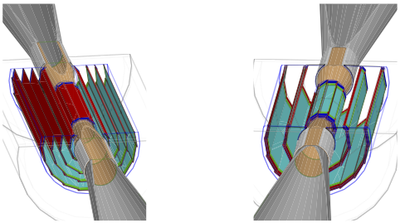
\includegraphics[width = 10 cm]{Pictures/vxd/ild_VXD.png}
     \caption{Overview of the two vertex detector option for the ILC. On the left, it is made of five single sided layers, whereas the right one represents three double-sided layers.}
   \end{figure}
   
   They are two different geometrical designs under studied to build the \gls{VXD}. 
   The first idea is to have a \gls{VXD} with five single-sided layers with a radii range from 15 to 60 mm.
   The other option is to have three double-sided layers, which will have pixel sensors on both side separated by a mechanical structure of 2 mm thickness. 
   The radii range is from 16 to 60 mm.
    
   Different detector technologies are under competition:

   \subsubsection{FPCCD}
   The \gls{FPCCD} has a small pitch {$\simeq 5 \mu\text{m}$} which gives a sub-micron spatial resolution and an excellent capability to separate two near tracks.
   In order to limit the charge spread, the $15 \mu\text{m}$ epitaxial layer (the sensitive volume) is completely depleted.

   \subsubsection{DEPFET}
    
    The \gls{DEPFET} is an active pixel detector in which field effect transistors are incorporated into each pixel.
    The sensor is completed depleted of free charged carries thanks to a voltage applied over the thickness.

    Rapid and efficient collection of signal on a deep implant underneath the field effect transistor
    Inside pixel: first amplification of signal
    Columns readout by two auxiliary \glspl{ASIC} while rows read out in rolling shutter mode.

   \subsubsection{CMOS}

   A third option is the integration of \gls{CMOS} pixel sensors. 
   The STAR experiment at RHIC is the first one to get an entire vertex detector made of ULTIMATE-MIMOSA28 CMOS sensors.
   One of the technology developed is described in section~\ref{sec:CMOS}.

  \section{PLUME}


  The \gls{PLUME} project is studying the feasibility to build double-sided vertex detector using \glspl{MAPS} sensors matching the \gls{ILC} requirements and is exploring the benefits of this design.
  A small collaboration involving three labs in the Europe, the IPHC-PICSEL of Strasbourg, the University of Bristol and the DESY-Hamburg lab, is studying that...

  

    \subsection{Design and goals}

    The figure~\ref{fig:PLUME} illustrate the design of a PLUME ladder.
    The mechanical structure is made of a 2 mm thick silicon-carbide foam which have a density varying between 8\% for the prototype build before 2011 and 4\% for the new ones.
    On each side, a low mass flex-cable is glued to power and to manage sensors from outside, via a connector on one edge.
    It is made of copper traces (prototype before 2011) or aluminum traces (new prototypes) coated in Kapton. 
    The ladder embeds twelve sensors, six on each face, that are glued and connected to the flex cable.
    At the moment, the design is dedicated to the MIMOSA-26 sensors but it could evolve to any kind of \gls{MAPS} sensors. 
    Although the MIMOSA-26 has a spatial resolution better than 3 $\mu$m, the integration time is not suited for the bunch train structures of the \gls{ILC}.

    The aims of the collaboration are to build ladders with a material budget better than 0.35 \% of $X_0$ for a spatial resolution better than 3 $\mu$m.

    \begin{figure}[!h]
      \centering
      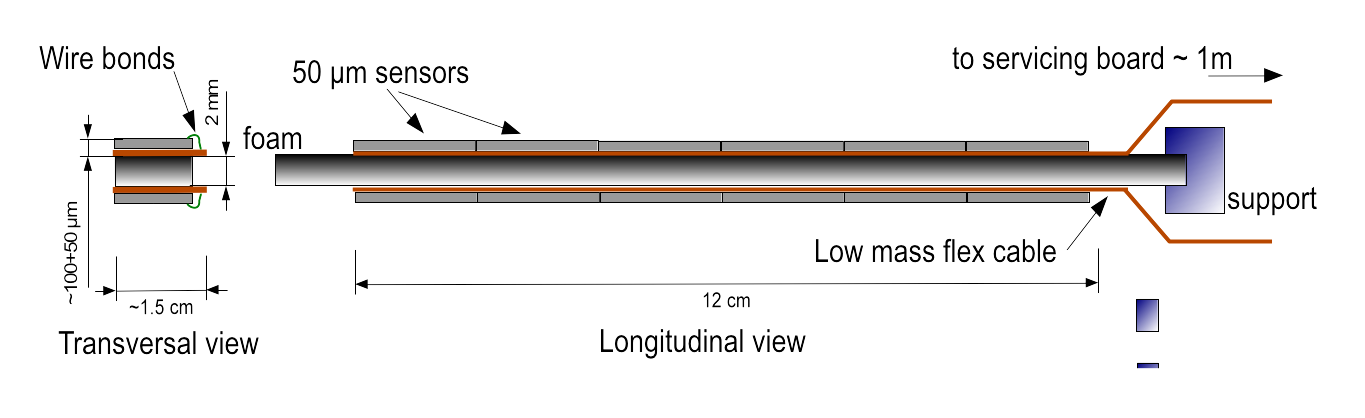
\includegraphics[width = 15 cm]{Pictures/vxd/plume_finalGoal.png}
      \label{fig:PLUME}
      \caption{Side view (transversal and longitudinal) of the PLUME mechanical structure.}
    \end{figure}

    \subsection{Prototypes}

    Before to reach the lightest ladder with a material budget of only 0.35 \%, the collaboration has studied the design, production and impact of the mechanical structure, but also how to power and control the sensors.
    
    The first ladder prototype (here labelled V0) was developed and test in 2009.
    It has two MIMOSA-20 analog output sensors on each side of a stiffener, providing a $1 \times 4 \text{ cm}^2$ sensitive area.
    As the purpose of this prototype was to settle the fabrication and the beam test procedure, the sensors and the flex-cables were not optimised.
     
    The second prototype featuring the final device design (V1) was developed in 2010. 
    The material budget is estimated to be 0.65 \% of $X_0$ in the sensor's sensitive area. 
    It is the first version to embed six MIMOSA-26 binary output sensors on each side of the stiffener that were working simultaneously.
    Two ladders were tested, one with 120 GeV pions at CERN-SPS in 2011 and the second one with positrons up to 5 GeV at DESY.
    The test beam at DESY is presented in chapter ... and some results of sensor's deformation observed at CERN are discussed in chapter ...

    The third prototype was mounted at the beginning of 2016 and has not been yet tested. 
    The traces thickness was reduced, the flex-cable width was adjust to the sensors width and the stiffener was made of a lower density Silicon Carbide foam reducing the material budget and the dead areas.

    \begin{table}
      \begin{center}
        \begin{tabular}{c c c c c c c}
        \hline %----------------------------
        \multirow{2}*{Layer}  & \multicolumn{3}{ c }{budget (\% X$_0$)}  \tabularnewline
                              &  V0 & V1 & Goal \tabularnewline
        \hline %----------------------------
        \hline %----------------------------
        Sensor                 & 0.053 & 0.053 & 0.053 \tabularnewline
        Flex                  & 0.524 & 0.150 & 0.034 \tabularnewline
        Passive components    & 0     & 0.033 & 0.033 \tabularnewline
        Stiffener (foam)      & 0.764 & 0.175 & 0.087 \tabularnewline
        Total                 & 1.926 & 0.654 & 0.334 \tabularnewline
        \hline %----------------------------
        \end{tabular}
        \label{tab:X0}
        \caption{Estimation of the material budget for the different prototypes of the PLUME ladder.}
      \end{center}
    \end{table}

    \subsection{Perspectives}

    Although the collaboration has shown their expertise to build light mechanical structures, more tests and optimisations have to be done.
    MIMOSA-26 sensors are not designed to match the \gls{ILC} specs. 
    The integration time of this sensor is 115.2 $\mu$s, whereas the bunch train last only 0.95 ms (bunch crossing spaced out by 337 ns), a new CPS with a faster integration time has to be built.
    Although some tests were performed to used the power pulsing on the Mi-26 in order to decrease the power consumption, this sensors can't be used for that purpose\todo{Reference to paper from Oleg}.  

    The collaboration has to perform power pulsing test in a strong magnetic field to study the impact of the Laplace forces on the ladder and also the impact of the power pulsing on the capacity of the sensors.

  
  \section{Integration of CMOS sensors}
  \label{sec:CMOS}

  Since the beginning of the 1990's, a new alternative to the \gls{CCD} was developed in the imaging industry: the \gls{APS} produced thanks to the \gls{CMOS} process.
  They are called active pixel sensors because the pixel is made of a photodiode  and an active amplifier. 
  This technology is well used in the industry and equipped most of the camera produced.

  The PICSEL group of the IPHC of Strasbourg is developing \gls{MAPS} for the particle physics community since 1999.
  They are called monolithic because the sensitive volume and the micro-electronic circuitry form one physical block.

  
    \subsection{Principle of a CMOS sensor}

    When a particle is traveling through matter, it loses energy via interaction with electrons and nuclei.
    For a thin layer of material, particles can cross all of the environment and lose a small fraction of their energy.
    It is admit that \gls{MIP} creates 80 e- per microns. 
    For thin layer energy lose describe by a Landau while thick material Gaussian.

    \subsection{Architecture}
    
    The \gls{CMOS} sensors developed by the IPHC of Strasbourg are called monolithic \gls{MAPS} sensors because the different layers of the sensor are made in one block of the same material.
    The structure of the sensor is highly doped P+ substrate made of a moderate quality silicon. 
    It means that their are a lot of defaults in the crystal structure.
    This implies a high recombination rate of charge carriers.
    Above the bulk a layer made of good quality silicon to avoid the recombination of the charge carriers is grown.
    It is low doped P- and is called epitaxial layer. 
    It is the sensitive part of the sensor. 
    On top of the epitaxial layer, a N-wells implant has the role of the charge collection.
    The junction between the N-wells and the epitaxial layer create a P-N junction.
    At this junction, a depleted area is created that attracts the charge carriers.
    Nevertheless, this P-N junction is only one part of the pixel.
    Next to the N-wells implants are sitting highly doped P-well that reflect the charge carriers to the N-wells implants. 
    The difference of doping between the bulk and the epitaxial layer is also used to reflect charge carriers to the collection implants.

    The typical doping concentration are $10^{15} \text{at/cm}^3$ for the epitaxial layer, $10^{19} \text{at/cm}^3$ in the substrate and $10^{17} \text{at/cm}^3$ for the other layers.
    The doping concentration defines the size of the depleted region.

    As no external voltage is applied on the sensor to increase the depleted region, the charge carriers by particles are thermally diffused inside the sensitive volume to the diode.
    Nevertheless, the different doping concentration produces a built-in voltage defined as: 

    \begin{equation}
      V_b = \frac{kT}{q}ln\left( \frac{N_{p+}}{N_{p-}}\right)
    \end{equation}
    
    The build-in voltage depends on the Boltzmann constant $k$, the temperature $T$, the elementary charge $q$ and the different concentrations doping $N_{p\pm}$ of the interface.
    The charge collection efficiency is different from a completed depleted sensor. 
    Indeed, the thermal diffusion 

    \begin{figure}
      \missingfigure{Sketch of CMOS sensor}
      \caption{Drawing of a CMOS sensor structure.}
    \end{figure}

    \begin{figure}
      \missingfigure{Electric sketch}
      \caption{Two different architectures of pixel. The left one is a pixel of type 3T, whereas the right one is a self-biased one.}
    \end{figure}

    \subsection{Using CMOS in HEP}

    The PICSEL group is developing \gls{MAPS} sensors for vertexing and tracking purposes in high energy experiment but for other fields.
    The vertex detector of the STAR experiment at RHIC is the first one ever using \gls{CMOS} sensor to take data during the whole campaign.
    
    The sensors used are the \gls{MIMOSA}-28/Ultimate chip, an extended version of the \gls{MIMOSA}-26, the chips that are equipping the telescope planes at DESY and CERN.

    \begin{figure}
      \missingfigure{Architecture of Mi26}
      \caption{Layout of the MIMOSA-26 matrix.}
    \end{figure}
